\chapter{Literature Review}
\label{cha:0}
\lipsum[79]

\section{Word2Vector Models}
The Word2Vector model builds high quality distributed vector representation of words from large corpus of millions of sentences. Each \textbf{word vector} is built from the sets of its context words (words appearing in the same sentence) hence they capture a lot of local semantic and syntactic information useful for several Natural Language Processing tasks. Two different type of models are used for building these word representations as introduced in \cite{Mikolov2013}. They are,
\begin{myitemize}
\item Skip Gram Model
    \begin{myitemize}
    \item \textbf{Training Objective:} Predict the Context words of the Center word
    \end{myitemize}
\item Continuous Bag of Words Model
\begin{myitemize}
    \item \textbf{Training Objective:} Predict the Center word from the Context words. 
    \end{myitemize}
\end{myitemize}

\subsection{Architecture of the Word2Vec Model}
The Item2Vector Neural Network is fully connected two layer Neural Network (One hidden layer and one output layer). The Input to the model is a one hot encoded vector of the center word and the expected output is a one hot encoded vector of the context words. Therefore the size of the input and the output layer is equal to the vocabulary of the corpus. The size of the hidden layer is much smaller than the size of the input/output layer, as we are expecting to learn high quality \textbf{low dimensional} vector representation of words.

\begin{figure}
  \centering
  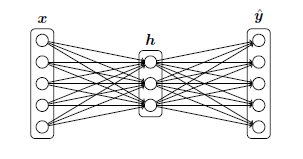
\includegraphics{2_1_NN_Architecture}
  \caption{A Simple Word2Vector Neural Network Architecture}
  \label{fig:1_1_NN_Architecture}
\end{figure}

\fref{fig:1_1_NN_Architecture} shows the architecture of a simple Word2Vector model. Unlike traditional Neural networks, the Word2Vec model does not include biases. It also employs only a linear activation function at the hidden layer. For each word two different distributed vector representations namely \textbf{input vector}  and the \textbf{output vector} are learnt. For example, for the word \textbf{book}, one input vector and one output vector is learnt. The reasons for this becomes obvious when we introduce the output probability estimation equation \ref{eqn:probestimate}. 

\paragraph*{A Description of the notations used in the equations:}
\begin{myitemize}
    \item \textbf{T} be the size of the vocabulary in the training corpus
    \item \textbf{x} be the input to the Neural network
    \item \textbf{N} be the size of the hidden layer
    \item \textbf{$\theta$} be the predicted score at the output layer
    \item \textbf{$\hat{y}$} be the predicted probability of the softmax classifier
    \item \textbf{y} be the true label at the output of the Neural network
    \item \textbf{V} be the weight matrix between the input and the hidden layer. It is of size \textbf{TxN}
    \item \textbf{U} be the weight matrix between the hidden and the output layer. It is of size \textbf{NxT}
\end{myitemize}

\paragraph*{A note on confusing nomenclature}
We can notice that the term input to the Neural network which is the vector \textbf{X} and the the input vector of the $i^{th}$ word \textbf{$u_i$} have the terms input in them. Similarly the output of the Neural network, the vector \textbf{$\theta$} and the output vector of the $j^{th}$ word \textbf{$v_j$} have the terms output in them. I understand that this is very confusing. But to stay consistent with the literature I have retained with this terminology. Each row of \textbf{V} represents the input vector representation of the corresponding word in the input layer and each column of the \textbf{U} represents the output vector representation of the corresponding word in the output layer. 

\fref{fig:1_2_Word2Vec_Architecture} shows the architecture of a simple Word2Vector model \cite{Rong2014}
\begin{figure}
  \centering
  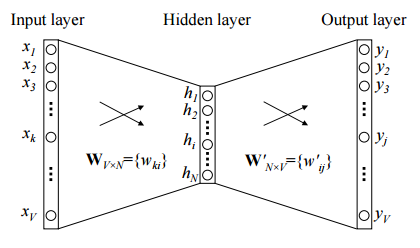
\includegraphics{1_2_Word2Vec_Architecture}
  \caption{A Simple Word2Vector Neural Network Architecture}
  \label{fig:1_2_Word2Vec_Architecture}
\end{figure}

\paragraph*{A Global Overview of modelling process}
Chunks of Math may interrupt the reader from getting a global idea of the whole modelling process. Hence I am presenting the global idea in a nutshell here, hoping that this will aid in better understanding of the following concept.

We are interested in deriving a distributed vector representation of words in our training corpus. For example, consider our training corpus consists of the following three sentences:
\begin{myitemize}
    \item Dog barks at the cat
    \item Cat eats the fish
    \item Caesar was a great king
\end{myitemize}

\begin{myenumerate}
\item Now we take up the first word \textbf{Dog} in the first sentence and encode it as a one hot encoded vector in the vocabulary of the corpus \ref{tab:dogtable}. 
\item Then we take up the words in the context within a window -m to +m and encode them as one hot encoded vector. Here in our case if we consider the context window of size 1, then we take up the word \textbf{barks} alone as context.
\item We propagate the one hot encoded input across the network and estimate the probability of each word in the vocabulary to be its context word.
\item Our training objective is to maximize the log likelihood of the context word given the current word i.e. $\textbf{p(context word|current word)}$ in case of skip-gram and the other way for CBOW.     
\end{myenumerate}

\begin{table}
  \centering
  \begin{tabular}{|c|c|c|c|c|c|c|c|}
  \hline
       Dog&barks&cat&eats&fish&Caesar&great&king  \\
       \hline
       1&0&0&0&0&0&0&0 \\
       \hline
  \end{tabular}
  \caption{One hot encoded vector of the word \textbf{Dog}}
  \label{tab:dogtable}
\end{table}






\subsection{Forward Propagation}
Remember \textbf{x} is the one hot encoded input to the neural network. In the forward propagation, the following computations are performed:

\begin{equation}
    \textbf{h} = \textbf{$v_{i}$}^T \textbf{x}
    \label{eqn:forwardprop1}
\end{equation}

\begin{equation}
    \textbf{$\theta$}=\textbf{$u_{j}$}^T \textbf{h}     
    \label{eqn:forwardprop2}
\end{equation}

We can see that essentially the equations \ref{eqn:forwardprop1} and \ref{eqn:forwardprop1} is just a dot product between the input vector of the $i^{th}$ word and the output vector of the $j^{th}$ word. The resulting \textbf{score} somehow intuitively tells us the un-normalized similarity of these two word vectors.

\subsection{Probability of the Output words}
Once we have computed the similarity scores between the input word and all the other words in the vocabulary, we can estimate the probability of the $j^{th} $ word being the context word when the $i^{th} $ word is the input word using the softmax function as follows:
\begin{equation}
    \hat{y_{ij}}=softmax(v_i*u_j)=softmax(\theta_{ij})
    \label{eqn:probestimate}
\end{equation}

\begin{figure}
  \centering
  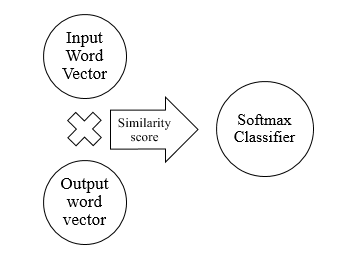
\includegraphics{1_3_Overall_process}
  \caption{Overall Word2Vector Model building process}
  \label{fig:1_3_Overall_process}
\end{figure}


\subsection{Training Objective}
The objective of the training is to maximize the log likelihood of the context word vector given the current word vector. 

\begin{equation}
    \hat{max} J(\theta)=\sum_{-m<j<m,j\neq0}{log(p(w_{c+j}|w_c))}
\end{equation}
\begin{equation}
    =\sum_{-m<j<m,j\neq0}{log(\hat{y}_{c,c+j})}
\end{equation}

\begin{equation}
    =\sum_{-m<j<m,j\neq0}{log(softmax(\theta_{c,c+j}))}
\end{equation}
\begin{equation}
    =\sum_{-m<j<m,j\neq0}{log(softmax(v_{c}^T u_{c+j}))}
    \label{eqn:objective4}
\end{equation}


Equation \ref{eqn:objective4} clearly shows that the objective of the training is to maximize the logarithm of the softmax classifier output, given the context word vector and the current word vector. The figure \ref{fig:1_3_Overall_process} also shows this clearly.

Following this, we have to learn the parameters of the model which will optimize the objective function. Generally Stochastic gradient techniques and Backpropagation algorithm are used for parameter update.

%%% Local Variables: 
%%% mode: latex
%%% TeX-master: "thesis"
%%% End: 
